\documentclass[a4paper, 12pt]{article}
\usepackage{amsmath} % for math functions
\usepackage{graphicx} % for linking images
\usepackage{float} % to force an inserted figure to stay in place
\usepackage{subcaption} % to display multiple figures side by side


% define the title
\author{Alina Zeng}
\title{\textbf{Is it lunchtime yet}}

% update May-28, 2021
% taking tutorial here at https://latex-tutorial.com/tutorials/first-document/




\begin{document}
% generates the title on a new page
\pagenumbering{gobble}   % to hide the page number on the cover page
\maketitle
\newpage
\pagenumbering{arabic}   % to unhide the page number


% the section commands are numbered and will appear in the table of contents of your document. Paragraphs aren’t numbered and won’t show in the table of contents
% insert the table of contents
\tableofcontents
\newpage  % making a new page for contents

\section{For Forever}
Dear Evan Hansen, today is going to be a great day and here is why. \newline
You can \textsl{lean} on me!
You can \textbf{count} on me~ \newline


\subsection{All we see is light, for forever}
Excited for Hamilton Tour in 2022. \newline

\subsubsection {{\small Small} is {\Large big}}
What's cookin'

\paragraph {What to do when you feel hungry}

\subparagraph {Time to eat out!} Have not had a chance in so long.

\section{Math Equations}
\paragraph {A few simple ones}
\begin{equation*}
  f(x) = x^2
\end{equation*}
% The automatic numbering is a useful feature, but sometimes it’s necessary to remove them for auxiliary calculations. LaTeX doesn’t allow this by default, now we want to include a package that does

\begin{equation*}
  1 + 2 = 3 
\end{equation*}

\begin{equation*}
  1 = 3 - 2
\end{equation*}

\subsection{Alignment}
\paragraph{Trying out alignment} ``=''
\begin{align*}
    f(x) &= x^2\\
    1 + 2 &= 3\\
  1 &= 3 - 2
\end{align*}
\subparagraph{LOL I don't quite like how this looks.}

\paragraph{Trying out alignment} ``2''
\begin{align*}
    1 + &2 = 3\\
  1 = 3 - &2
\end{align*}
\subparagraph{This is a bit funky.}


\subsection{Would you like some more}
\paragraph{Some simple LaTeX math functions}
\begin{align*}
  f(x) &= x^2\\
  g(x) &= \frac{1}{x}\\
  y(x) &= \left(\frac{1}{\sqrt{x}}\right)\\
  F(x) &= \int^a_b \frac{1}{3}x^3
\end{align*}
\subparagraph{More sophisticated functions can happen by combining various commands}



\subsection{Trying out matrices}
\subparagraph{Matrices inside parentheses}
\begin{equation*}
A = 
\begin{pmatrix}
1 & 2 & 3 \\
4 & 5 & 6 \\
7 & 8 & 9
\end{pmatrix}
\end{equation*}

\subparagraph{Matrices without brackets}
\begin{equation*}
   \begin{matrix} 
   a_{11} & a_{12} & a_{13}  \\
   a_{21} & a_{22} & a_{23}  \\
   a_{31} & a_{32} & a_{33}  \\
   \end{matrix} 
\end{equation*}

\subparagraph{Matrices have to happen within the equation environment}
\begin{equation*}
\begin{matrix}
1 & 0\\
0 & 1
\end{matrix}
\end{equation*}

\subparagraph{Some more varieties}
\begin{equation*}
   \begin{vmatrix} 
   a_{11} & a_{12} & a_{13}  \\
   a_{21} & a_{22} & a_{23}  \\
   a_{31} & a_{32} & a_{33}  \\
   \end{vmatrix} 
\end{equation*}

\subparagraph{Here are examples with matrix 2x2 with pmatrix, bmatrix, vmatrix, Vmatrix environments:}
\begin{equation*}
\begin{matrix} 
a & b \\
c & d 
\end{matrix}
\quad  % side by side
\begin{pmatrix} 
a & b \\
c & d 
\end{pmatrix}
\quad
\begin{bmatrix} 
a & b \\
c & d 
\end{bmatrix}
\quad
\begin{vmatrix} 
a & b \\
c & d 
\end{vmatrix}
\quad
\begin{Vmatrix} 
a & b \\
c & d 
\end{Vmatrix}
\end{equation*}

\subparagraph{Small matrix environment} For more, refer to \textsl{https://www.math-linux.com/latex-26/faq/latex-faq/article/how-to-write-matrices-in-latex-matrix-pmatrix-bmatrix-vmatrix-vmatrix} \\
\begin{center}
\textbf{I love small matrices such as$\big(\begin{smallmatrix} a & b\\ c & d \end{smallmatrix}\big)$}
\end{center}

\section{Captioned Images in LateX}
\subsection{Temperature of Boston}
\begin{figure}[H]  % The float package (\usepackage{float}) allows to set the option to [H], which is even stricter than [h!].
  \includegraphics[width=\linewidth]{Figures/Temp_complete_2015.png}
  \caption{Temperature plot made using ggplot2, May 28 2021}
  \label{fig:Temp_complete_20151}
\end{figure}
Figure \ref{fig:Temp_complete_20151} shows temperature plot.

\paragraph{} At some point, you will notice that the figure doesn’t necessarily show up in the exact place as you put your code in the .tex file. If your document contains a lot of text, it’s possible that LaTeX will put the picture on the next page, or any other page where it finds sufficient space. To prevent this behavior, it’s necessary to set the \textbf{float} value for the figure environment.

\subsection{Adding multiple subfigure environments within a figure environment.}
\begin{figure}[h!]
  \centering
  \begin{subfigure}[b]{0.45\linewidth}
    \includegraphics[width=\linewidth]{Figures/improved_resolution_thanlyou_cairo.png}
    \caption{Mean plot.}
  \end{subfigure}
  \begin{subfigure}[b]{0.45\linewidth}
    \includegraphics[width=\linewidth]{Figures/improved_resolution_thanlyou_cairo.png}
    \caption{More mean plot.}
  \end{subfigure}
  \caption{The same mean plot. Two times.}
  \label{fig:meanplot}
\end{figure}
\newpage

\newpage
\subsubsection{Too much coffee?}
\begin{figure}
  \centering
  \begin{subfigure}[b]{0.3\linewidth}
    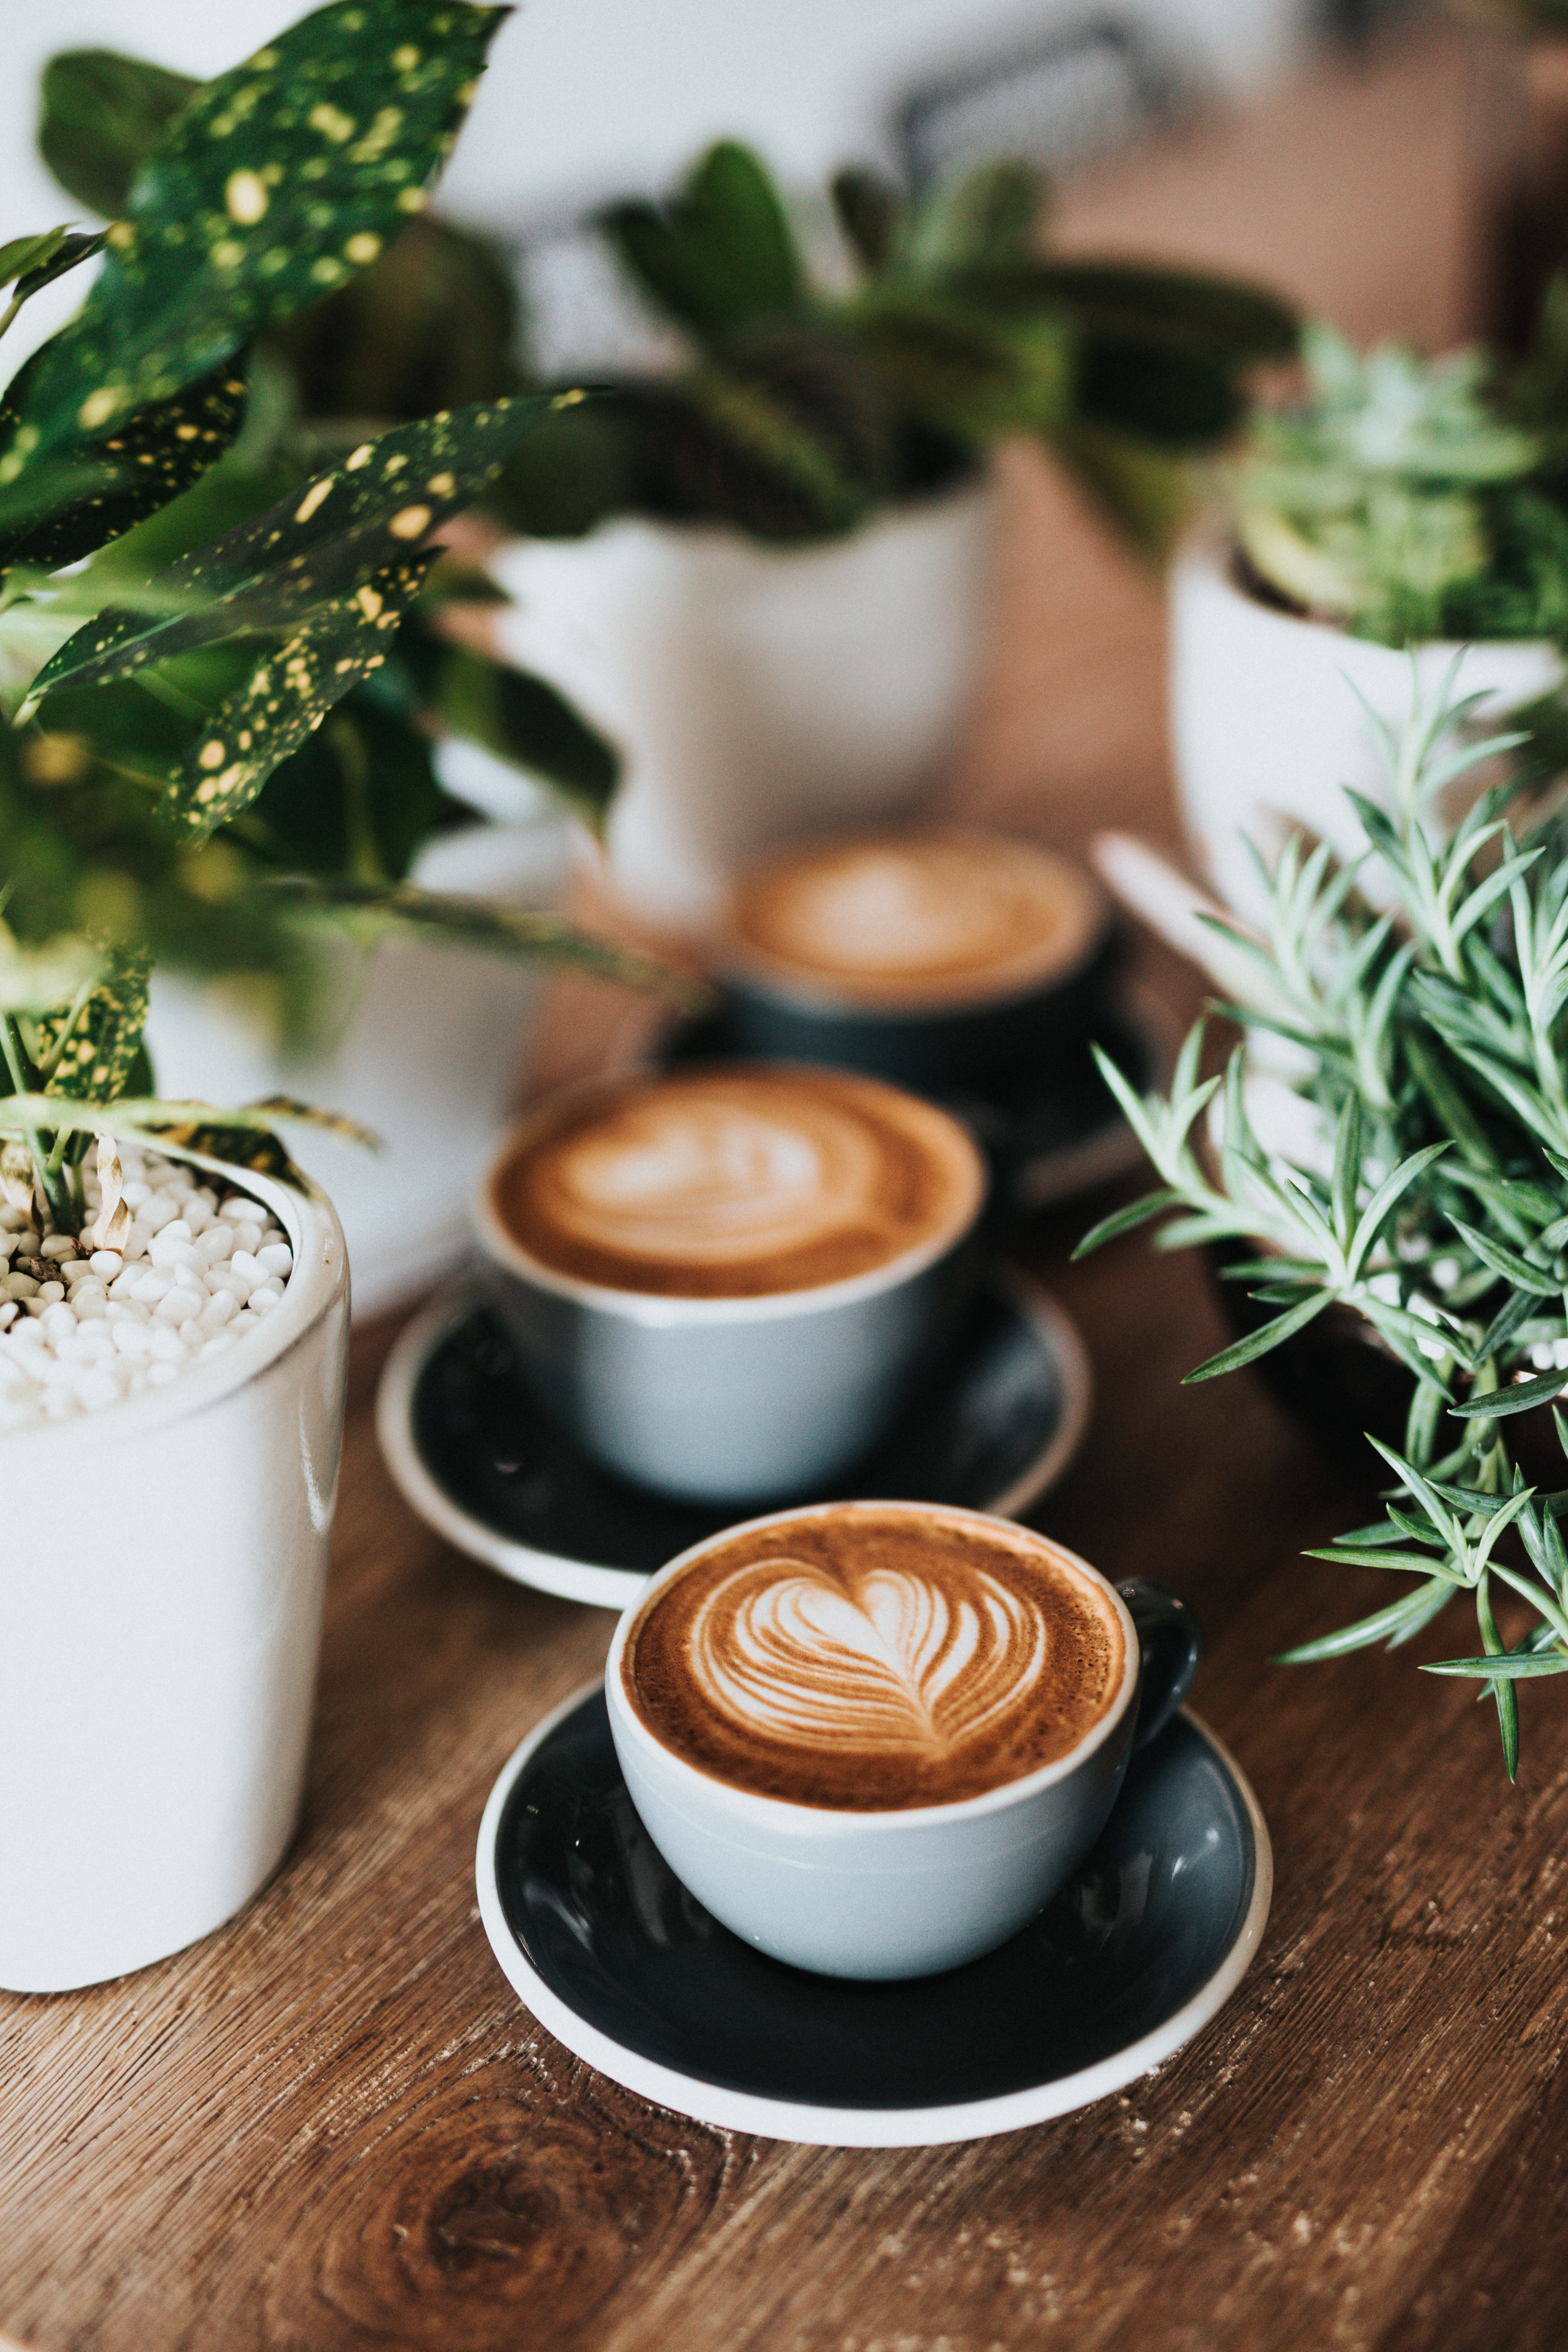
\includegraphics[width=\linewidth]{Figures/nathan-dumlao-zUNs99PGDg0-unsplash.jpg}
     \caption{Coffee.}
  \end{subfigure}
  \begin{subfigure}[b]{0.3\linewidth}
    \includegraphics[width=\linewidth]{Figures/devin-avery-5iRgh_G0eRY-unsplash.jpg}
    \caption{More coffee.}
  \end{subfigure}
  \begin{subfigure}[b]{0.3\linewidth}
    \includegraphics[width=\linewidth]{Figures/clay-banks-_wkd7XBRfU4-unsplash.jpg}
    \caption{Tasty coffee.}
  \end{subfigure}
  \begin{subfigure}[b]{0.8\linewidth}
    \includegraphics[width=\linewidth]{Figures/nathan-dumlao-6VhPY27jdps-unsplash.jpg}
    \caption{Too much coffee.}
  \end{subfigure}
  \caption{Lots of coffee and I don't even like coffee. \textsl{Images sourced from Unsplash}.}
  \label{fig:coffee3}
\end{figure}
\newpage


\section{Ending}
\ldots{} and here it ends.

\paragraph{will continue tmrw} at https://latex-tutorial.com/tutorials/amsmath/
\end{document}
